\documentclass{article}
\usepackage[utf8]{inputenc}
\usepackage[margin=2cm]{geometry}
\usepackage{fullpage,enumitem,amssymb,amsmath,xcolor,cancel,gensymb,hyperref,graphicx}
\usepackage[brazilian]{babel}
\usepackage{indentfirst}
\usepackage{graphicx}
\usepackage{caption}
\usepackage{tabularx}
\usepackage{array}
\usepackage{float}
\usepackage{booktabs, multirow}

\begin{document}
\begin{center}
    \textbf{\LARGE MAP2212 - Laboratório de Computação e Simulação}\\
    \vspace{0.3cm}
    \textbf{\Large Relatório - EP02}\\
    \vspace{0.3cm}
    \large{Vítor Garcia Comissoli - 11810411}
\end{center}

\section{Introdução}
    
    O objetivo deste EP é a estimação da integral $\gamma$ da $f(x)$ estipulada pelo enunciado por meio de quatro métodos de Monte Carlo, sendo eles \textbf{Crude}, \textbf{Hit or Miss}, \textbf{Control Variate} e \textbf{Importance Sampling}, de modo que a estimativa para $\gamma$ obitida tenha um erro de, no máximo, 0.05\% de $\gamma$, com 95\% de confiança, ou seja, que fique dento do Intervalo de Confiança $[\gamma\cdot(1 - 0.0005),\gamma\cdot(1 + 0.0005)]$ com $\alpha=0.95$.\\
    \\
    Vale ressaltar também que, neste EP, deve-se tratar o valor da integral $\gamma$ como desconhecido, então todas as contas devem ser realizadas com um estimador qualquer para $\gamma$ ($\hat{\gamma}$).
    
\section{Discussão Teórica}
    
    Primeiramente, foi necessário descobrir o valor de \textbf{n} (número de loopings realizados pela função "for in range") para que as estimativas de $\gamma$ se encontrem dentro do intervalo de confiança dado acima com $\alpha = 0.95$\\
    \\
    Para isso, foi utilizada a aproximação assintótica para uma Normal(0,1). Disso temos que a fórmula para a obtenção de cada um dos quatro valores de \textbf{n} (um para cada método) pode ser dada por:\\
    $$n \geq \frac{z_\alpha¨2 \cdot \sigma^2}{\epsilon^2} \Leftrightarrow \frac{z_\alpha \cdot \sigma}{\sqrt{n}} \leq \epsilon $$
    \\
    Como temos um $\alpha=0.95$, tomamos pela tabela da normal que $z_\alpha = 1.96$\\
    \\
     Temos que $\epsilon = \gamma \cdot0.0005$. Pode-se dizer que o erro no quadrante se dá por:\\
    $$ |\hat{\gamma}-\gamma| \leq 0.0005\cdot \hat{\gamma}$$
    Disso, dizemos que o erro experimental a ser usado na fórmula da aproximação assintótica se dá por
    $\epsilon = 0.0005\cdot \hat{\gamma}$, sendo $\hat{\gamma}$ um estimador para $\gamma$ que será encontrado a seguir.\\
    \\
    Sabemos pelo enunciado, que a função $f(x)$ se dá por:\\
    $$ f(x) = e^{-Ax}\cdot cos(Bx) $$
    Como, pelo enunciado, $A = 0.RG$ e $B = 0.CPF$:\\
    $$ f(x) = e^{-0.54018912x}\cdot cos(0.509920698x) $$
    Plotando o gráfico de $f(x)$ no intervalo $[0,1]$ temos a seguinte função:
    \begin{figure}[H]
        \centering
        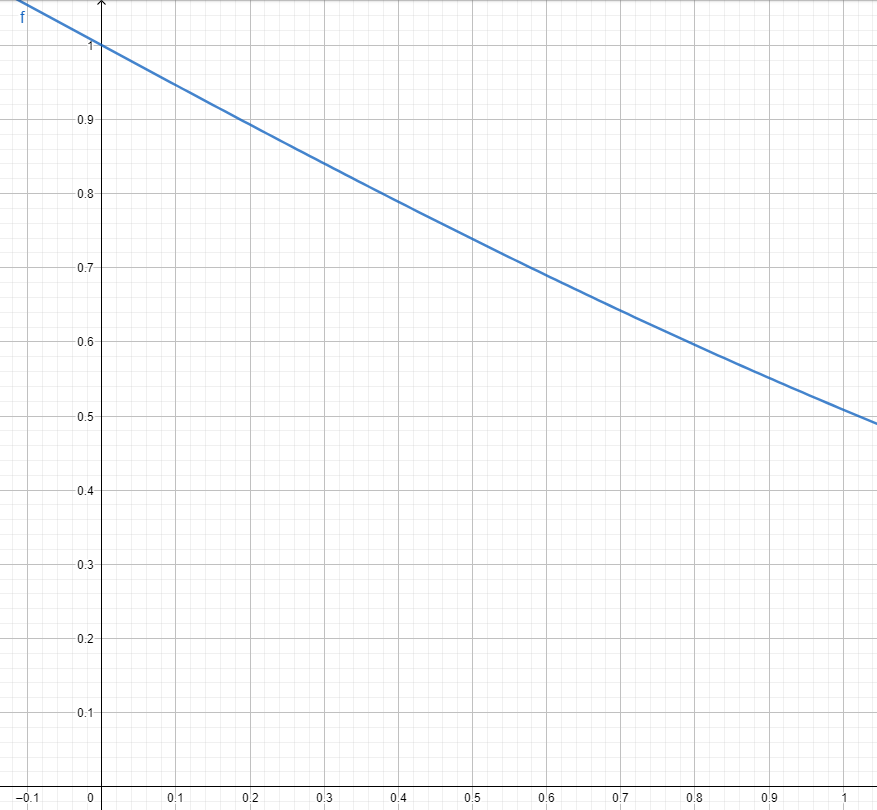
\includegraphics[width=.75\textwidth]{gráfico f(x).png}
        \caption{Gráfico da Função $f(x)$ no intervalo $[0,1]$}
        \label{fig:grafico}
    \end{figure}
    Pelo gráfico, e por saber que o exponte da exponencial é negativo, temos que a função é decrescente no intervalo $[0,1]$, o que implica que:
    $$f(1) \leq \gamma \leq f(0) \Leftrightarrow 0.50852 \leq \gamma \leq 1$$ Sabendo disso, podemos assumir $\hat{\gamma} = 0.50852$, já que quanto menor o valor de $\hat{\gamma}$, maior o valor de \textbf{n}, o que implica em um estimador para a integral ainda mais preciso que o enunciado pelo exercício.Tendo isso, podemos agora encontrar o valor de \textbf{n} nos quatro casos.\\
    \\
    Calculemos agora o valor de \textbf{n} para cada um dos quatro métodos:

\subsection{Crude}

A variância para esse método, segundo o slide de aula, pode ser dada por:
$$ \sigma^2_c = \frac{1}{n} \int_{a}^{b} (f(x) - \gamma)^2 dx $$
Nesse caso específico, a variância se dá por:
$$ \sigma^2 = \int_{0}^{1} (f(x) - \hat{\gamma})^2 dx \Leftrightarrow \int_{0}^{1} (e^{-0.54018912x}\cdot cos(0.509920698x) - 0.50852)^2 dx $$
$$ \Rightarrow \sigma^2 \approx 0.07575 $$
\\
Agora, tendo todos os valores, podemos encontrar o valor de n desejado utilizando a fórmula da aproximação assintótica para uma Normal(0,1) já apresentada acima. Temos então:\\
    
    $$\frac{z_\alpha \cdot \sigma}{\sqrt{n}} \leq \epsilon \Leftrightarrow \frac{1.96 \cdot\sqrt{0.07575}}{\sqrt{n}} \leq 0.0005\cdot 0.50852$$\\
    
    $$\Leftrightarrow \sqrt{n}\geq \frac{1.96\cdot 0.27522}{0.00025426}\Leftrightarrow \sqrt{n}\geq 2122 \Leftrightarrow n\geq 4502884$$\\
    \\
    Temos assim, que o valor de \textbf{n} a ser colocado no programa para satisfazer as condições impostas pelo enunciado deve ser igual a 4502884.

\subsection{Hit or Miss}

A variância para esse método, segundo o slide de aula, pode ser dada por:
$$ \sigma^2_h = \frac{\gamma\cdot(1-\gamma)}{n} $$
Nesse caso específico, a variância se dá por:
$$ \sigma^2 = \hat{\gamma}\cdot(1-\hat{\gamma}) \Leftrightarrow 0.50852 \cdot (1-0.50852) \Leftrightarrow 0.50852 \cdot 0.49148 $$
$$ \Rightarrow \sigma^2 \approx 0.24993 $$
\\
Agora, tendo todos os valores, podemos encontrar o valor de n desejado utilizando a fórmula da aproximação assintótica para uma Normal(0,1) já apresentada acima. Temos então:\\
    
    $$\frac{z_\alpha \cdot \sigma}{\sqrt{n}} \leq \epsilon \Leftrightarrow \frac{1.96 \cdot\sqrt{0.24993}}{\sqrt{n}} \leq 0.0005\cdot 0.50852$$\\
    
    $$\Leftrightarrow \sqrt{n}\geq \frac{1.96\cdot 0.49992}{0.00025426}\Leftrightarrow \sqrt{n}\geq 3854 \Leftrightarrow n\geq 14853316$$\\
    \\
    Temos assim, que o valor de \textbf{n} a ser colocado no programa para satisfazer as condições impostas pelo enunciado deve ser igual a 14853316.

\subsection{Control Variate}

A variância para esse método, segundo o slide de aula, pode ser dada por:

$$Var(\hat{\gamma}) = \frac{1}{n} \cdot (\sigma^2(f(x_i)) + \sigma^2(\varphi(x_i))-2\rho(f(x_i),\varphi(x_i))\sigma(f(x_i))\sigma(\varphi(x_i))$$

Como não posuímos todos os dados necessários para calcularmos a variância desse método pela equação acima, utilizaremos a variância amostral para calcular o valor de \textbf{n}.\\
\\
Ultilizando um $\hat{n} = 100000$ no código, e repetindo esse processo 100 vezes, obteve-se as estimativas para média e variância de forma amostral, sendo $\mu_a = 0.743915$ e $\sigma^2_a = 2.57\cdot 10^{-10} $.\\
\\
Como a variância amostral obtida é muito baixa, temos que com o próprio $\hat{n} = 100000$ a estimativa para $\gamma$ já dá dentro do intervalo de acurácia, então tomemos $n = \hat{n} = 100000$

\subsection{Importance Sampling}

A variância para esse método, segundo o slide de aula, pode ser dada por:
$$ \sigma^2_s = \frac{1}{n} \int (\frac{f(x)}{g(x)} - \gamma)^2 \cdot g(x) dx $$
Nesse caso específico, a variância se dá por:
$$ \sigma^2 = \int_{0}^{1} (\frac{f(x)}{g(x)} - \hat{\gamma})^2 \cdot g(x) dx \Leftrightarrow $$
$$\Leftrightarrow \int_{0}^{1} (\frac{e^{-0.54018912x}\cdot cos(0.509920698x)}{g(x)}-0.50852)^2\cdot g(x) dx$$

Como g(x) é a função densidade de probabilidade (fdp) de uma beta(1,1.2), temos que:

$$ g(x)=\frac{\Gamma(a+b)}{\Gamma(a)\cdot \Gamma(b)} x^{(a-1)}\cdot (1-x)^{(b-1)} \Leftrightarrow1.2 \cdot (1-x)^{(0.2)}$$

Assim:

$$ \sigma^2 = \int_{0}^{1} (\frac{e^{-0.54018912x}\cdot cos(0.509920698x)}{1.2 \cdot (1-x)^{(0.2)}}-0.50852)^2\cdot 1.2 \cdot (1-x)^{(0.2)} dx$$
$$ \Rightarrow \sigma^2 \approx 0.0596348 $$

Agora, tendo todos os valores, podemos encontrar o valor de n desejado utilizando a fórmula da aproximação assintótica para uma Normal(0,1) já apresentada acima. Temos então:\\
    
    $$\frac{z_\alpha \cdot \sigma}{\sqrt{n}} \leq \epsilon \Leftrightarrow \frac{1.96 \cdot\sqrt{0.0596348}}{\sqrt{n}} \leq 0.0005\cdot 0.50852$$\\
    
    $$\Leftrightarrow \sqrt{n}\geq \frac{1.96\cdot 0.24420}{0.00025426}\Leftrightarrow \sqrt{n}\geq 1882 \Leftrightarrow n\geq 3541924$$\\
    \\
    Temos assim, que o valor de \textbf{n} a ser colocado no programa para satisfazer as condições impostas pelo enunciado deve ser igual a 3541924.

\section{Discussão do Código}

Os prints abaixo do código estão comentados linha por linha, explicitando todos os processos tomados.

    \begin{figure}[H]
        \centering
        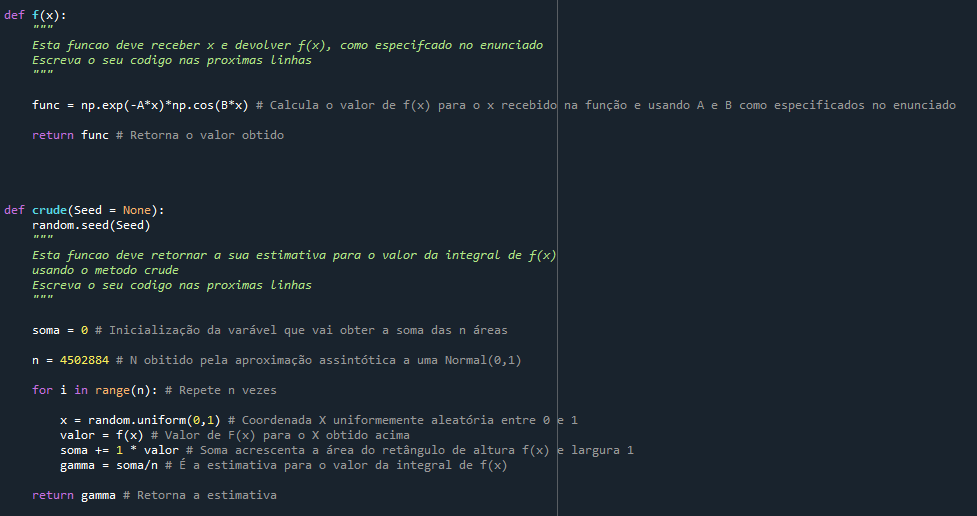
\includegraphics[width= 1 \textwidth]{Código f(x) e crude.png}
        \caption{Código e comentários das funções f(x) e Crude}
        \label{fig:grafico}
    \end{figure}
    
    \begin{figure}[H]
        \centering
        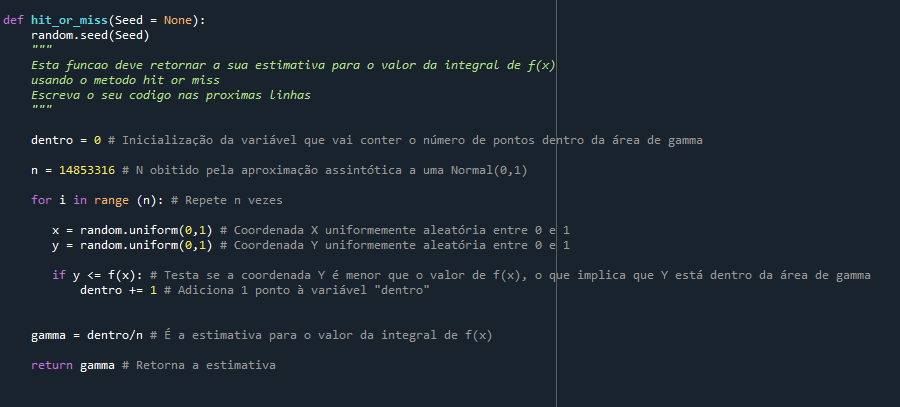
\includegraphics[width= 1 \textwidth]{Código hit or miss.png}
        \caption{Código e comentários da função Hit or Miss}
        \label{fig:grafico}
    \end{figure}

    \begin{figure}[H]
        \centering
        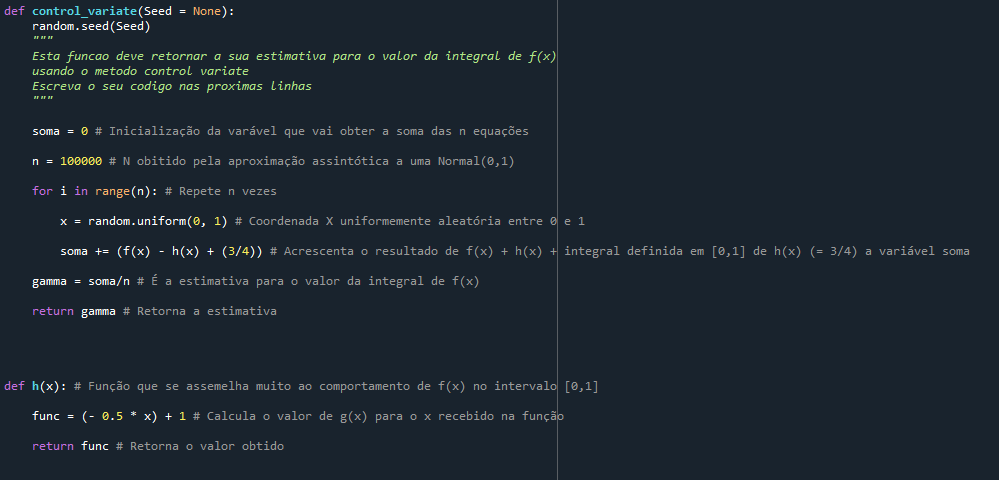
\includegraphics[width= 1 \textwidth]{Código control variate.png}
        \caption{Código e comentários da função Control Variate}
        \label{fig:grafico}
    \end{figure}
    
    \begin{figure}[H]
        \centering
        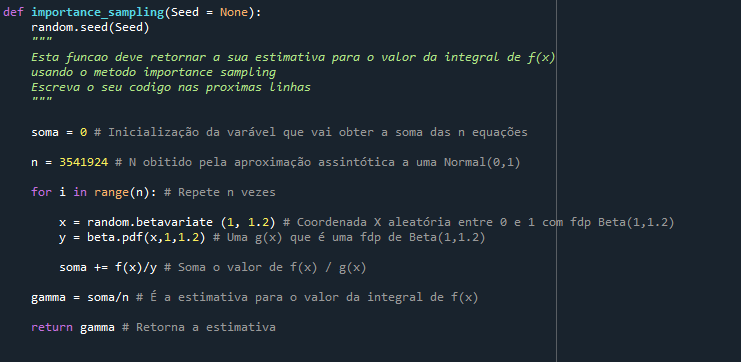
\includegraphics[width= 1 \textwidth]{Código importance sampling.png}
        \caption{Código e comentários da função Importance Sampling}
        \label{fig:grafico}
    \end{figure}


\section{Resultado}

O teste dos resultados foi realizado pela criação de uma função main() que chama as funções dos quatro métodos \textbf{n} vezes e imprime a razão das estimativas para $\gamma$ que se encontram dentro do intevalo de confiança sobre o número total de estimativas realizadas.\\
\\
No método Crude, para $n = 50$, essa razão foi de $1.0$, com média $\mu = 0.74392$. O tempo gasto para um loop de $n = 50$ foi de, aproximadamente, $832.59$ segundos ($13.88$ min).\\
\\
Já no método Hit or Miss, para um $n = 50$, a razão obtida também foi de $1.0$, com média $\mu = 0.74390$. O tempo gasto para um loop de $n = 50$ foi de, aproximadamente, $2522.23$ segundos ($42.04$ min).\\
\\
No método Control Variate, para $n = 50$, essa razão foi de $1.0$, com média $\mu = 0.74392$. O tempo gasto para um loop de $n = 50$ foi de, aproximadamente, $17.90$ segundos.\\
\\
Por fim, no método Important Sampling, para $n = 30$, essa razão foi de $1.0$, com média $\mu = 0.74392$. O tempo gasto para um loop de $n = 50$ foi de mais de 3 horas.\\
\\
Todos os valores apresentados acima mostram-se coerentes aos parâmetros de acurácia $\alpha = 0.95$ e $\epsilon = \gamma \cdot0.0005$, estipulados pelo enunciado do EP. \\
\\
Com isso podemos concluir que o resultado obtido foi dentro do esperado.

\section{Conclusão}

Como já dito previamente, todos o métodos se mostraram coerentes aos parâmetros de acurácia de $\alpha = 0.95$ e $\epsilon = \gamma \cdot0.0005$. Contudo, a outros fatores que podem ser analisados.\\
\\
Analisando quanto a performance computacional temos que o método de Important Sampling se mostrou muito lento e custoso quando comparado com os outros 3 métodos, seguido pelo método Hit or Miss, o método Crude e, por fim, o método Control Variate, que se mostrou o mais eficiente.\\
\\
Quanto ao tamanho das variâncias, tivemos Control Variate com a menor variância de todos os métodos, e Hit or Miss com maior variabilidade.\\
\\
Por fim, quanto ao tamanho do \textbf{n} encontrado, temos que o método Hit or Miss necessitou do maior valor de n, enquanto o método Control Variate  foi o que utilizou o menor valor de n dos quatro.

\end{document}